\documentclass[output=paper]{LSP/langsci} 
\author{Marisa Lousada\affiliation{Universidade de Aveiro e CINTESIS.UA}\and 
Dina Caetano
Alves\affiliation{Instituto Politécnico de Setúbal e Centro de Linguística da Universidade de Lisboa}\lastand 
Maria João Freitas\affiliation{Universidade de Lisboa, Faculdade de Letras, Centro de Linguística}
}
\title{Avaliação linguística em contextos de desenvolvimento típico e atípico: aspetos fonéticos e fonológicos}  
\rohead{\thechapter\hspace{0.5em}Avaliação linguística em contextos de desenvolvimento típico e atípico}
\abstract{\noabstract}
\ChapterDOI{10.5281/zenodo.889445}
\maketitle
\begin{document}
\section{Avaliação fonética e fonológica: perspetiva histórica}
\label{sec:lousada_avaliacao}

Até à década de 70, as crianças com um discurso ininteligível eram usualmente diagnosticadas com perturbação articulatória e submetidas a uma intervenção articulatória tradicional, como a proposta em \citet{vanriper1939}. Em 1976, com o trabalho de \cite{ingram1976}, assiste-se a uma mudança de paradigma, da \textit{articulação} para a \textit{fonologia}. Assume-se, assim, que as dificuldades na produção poderão decorrer, não de dificuldade articulatória na efetiva produção de sons individuais, mas antes de um problema linguístico, portanto, cognitivo e não motor, relativo à constituição e organização do sistema fonológico, no qual se incluem os fonemas, que contribuem para a atribuição de significado \citep{baker2006}. Esta mudança teve repercussões no diagnóstico, na avaliação e na intervenção terapêutica. Crianças que, anteriormente, apresentavam diagnóstico de perturbação articulatória passam a ser diagnosticadas com \isi{perturbação fonológica}. Em termos do processo de avaliação, também ocorreram alterações substanciais. As amostras de fala eram analisadas segmento a segmento e os erros classificados enquanto `substituições, omissões, distorções e adições' de segmentos (análise SODA) \citep{bowen2015}. Com esta mudança de paradigma, a análise de base fonológica passa ainda a identificar padrões inerentes às dificuldades observadas (e.g., o fonema \textipa{/z/} produzido como \textipa{[s}] e o \textipa{/Z/} produzido como \textipa{[S]} indicam o mesmo padrão de erro, associado à preferência por segmentos não vozeados) \citep{baker2006}. Diferentes tipos de análise fonológica são utilizados, sendo a proposta de \cite{stampe1979}, relativa ao uso de \isi{processos fonológicos} enquanto instrumentos descritivos dos padrões de erro, uma das mais utilizadas na atualidade.

Relativamente aos princípios da intervenção, também se verificaram alterações. Na perspetiva articulatória, o objetivo geral da intervenção centrava-se essencialmente na articulação de sons individuais, ou seja, no treino da produção motora dos mesmos \citep{vanriperemerick1984}. Numa perspectiva fonológica, a intervenção visa a reabilitação do sistema fonológico da criança \citep{baker2006}, do domínio da cognição. 

Nos últimos anos, a classificação das perturbações que afetam o sistema sonoro das produções de fala vai além da dicotomia articulação \textit{versus} fonologia, tendo dado origem à proposta de diferentes subgrupos de perturbações \citep{dodd2005understanding,shriberg_etal2010,stackhousewells1997}. No entanto, não existe um consenso entre os investigadores quanto à melhor classificação a utilizar \citep{waringknight2013}. 

\textit{Perturbações dos Sons da Fala} (PSF)\is{perturbações dos sons da fala}, ou \textit{Speech Sound Disorders}, é a expressão genérica utilizada atualmente para designar as várias perturbações que podem ocorrer no campo da articulação ou da fonologia \citep{apa2013}. Os investigadores têm verificado que as crianças com estas perturbações constituem um grupo heterogéneo, com diferentes níveis de gravidade, causas subjacentes e/ou tipos de erro (característicos ou não), com comprometimento, ou não, de outros domínios linguísticos e com diferentes tipos de resposta ao tratamento. Algumas PSF decorrem de causas conhecidas como a perturbação do desenvolvimento intelectual, a perda auditiva neurossensorial, a fenda lábio-palatina ou a paralisia cerebral, no entanto, para a maioria, não existe uma causa conhecida \citep{waringknight2013}.

Ao longo dos anos, as orientações fornecidas para a avaliação das alterações da fala têm acompanhado as diferentes definições propostas para este tipo de dificuldades, ora dando mais ênfase à sua etiologia \citep{shriberg_etal2010}, ora às suas características linguísticas \citep{broomfielddodd2004}. De entre estas, assiste-se a uma oscilação entre o papel da fonética e o da fonologia, o que nos remete para uma reflexão em torno dos contributos da Linguística nesta\largerpage matéria, a fim de clarificar aspetos epistemológicos relativos a esta patologia.

\section{Contributos da Linguística para a \isi{avaliação fonológica}}
\label{sec:lousada_contributos}

A Linguística constitui uma das várias áreas do saber convocadas para a prática clínica e para a investigação desenvolvidas por terapeutas da fala. Inversamente, estudos disponibilizados por estes profissionais têm permitido testar hipóteses sobre a organização da informação linguística no cérebro. As duas áreas de trabalho interagem, assim, ativamente, no sentido da consolidação do conhecimento sobre as operações cognitivas associadas ao processamento linguístico.

No caso dos estudos sobre aquisição da linguagem, estes têm disponibilizado dados provenientes dos domínios da perceção e da produção que permitem: 

\begin{enumerate}[label=(\roman*)]
\item \textit{definir ordens de aquisição das unidades linguísticas} (por exemplo, a estrutura silábica CV ( \textit{pá} \textipa{[\textprimstress pa]}) precede a estrutura CVC (\textit{pés} \textipa{[\textprimstress pES]}); os segmentos com pontos de articulação anteriores (bilabial, labiodental, dental, alveolar) tendem a preceder os posteriores (palatal, velar, uvular)); 

\item identificar padrões linguísticos específicos dos desempenhos verbais infantis, ausentes nos adultos (por exemplo, os grupo consonânticos sofrem redução (braço \textipa{[\textprimstress brasu]} $\rightarrow$ \textipa{[\textprimstress baSu]} João (2;4.30)) e os segmentos vozeados tendem a ser substituídos por não vozeados). 
\end{enumerate}

Alguns destes aspetos são universais, nomeadamente os referidos nos pontos acima, e outros são específicos de dadas línguas naturais, como, por exemplo, o uso de Ataques vazios nas primeiras produções infantis (\textit{jipe} \textipa{[Zíp1]} $\rightarrow$ \textipa{[ípi]} João (2;2.28); cf. Capítulo 4 neste volume). A avaliação linguística efetuada em contexto clínico tem, assim, como referência as descrições dos perfis linguísticos de crianças com desenvolvimento típico, que permitem a identificação de situações de desenvolvimento atípico em crianças com patologias indiciadas por alterações do comportamento verbal. 

\subsection{Distinção entre Fonética e Fonologia}
\label{subsec:lousada_distincao}

Referimos, acima, os papéis distintos da Fonética e da Fonologia na avaliação do desenvolvimento linguístico em contextos típico e atípico: a Fonética está mais associada a problemas articulatórios, de natureza motora, e a Fonologia, a problemas de organização da informação linguística no sistema cognitivo da criança. A componente da gramática que designamos como \textit{Fonologia} estabelece relações estreitas com a \textit{Fonética}; a dificuldade em distinguir unidades e procedimentos associadas a ambas as áreas decorre do facto de ambas usarem recursos terminológicos comuns. 

Distinguimos entre unidades segmentais que usamos para representar o conhecimento fonológico (por exemplo, os \textit{fonemas}), do domínio da cognição, e unidades segmentais que constituem os \textit{outputs} fisicamente mensuráveis dessas unidades (por exemplo, os \textit{fones}), do domínio da Física. Os \textit{fonemas} são, assim, \textit{unidades abstratas} que usamos para representar o conhecimento sobre as unidades sonoras da língua, conhecimento esse armazenado no cérebro, portanto, do plano do processamento cognitivo central. Os fones são \textit{unidades físicas}, do plano da execução periférica: estas unidades são produto da ativação motora dos articuladores (unidades articulatórias), são transmitidas sob a forma de ondas sonoras (unidades acústicas) e captadas mecanicamente pelo aparelho auditivo, após o que são conduzidas ao sistema nervoso central, através do sistema nervoso periférico. Sempre que quisermos referir as unidades mínimas da cadeia sonora, sem remeter para os níveis fonológico ou fonético, poderemos utilizar o termo \textit{segmento}, presente na literatura para referir esta unidade sonora, em geral, independentemente do seu estatuto linguístico (\textit{fonema} ou \textit{fone}). Veja-se o diagrama na figura \ref{fig:lousada_1}, que representa o que acabámos de expor:

\begin{figure}
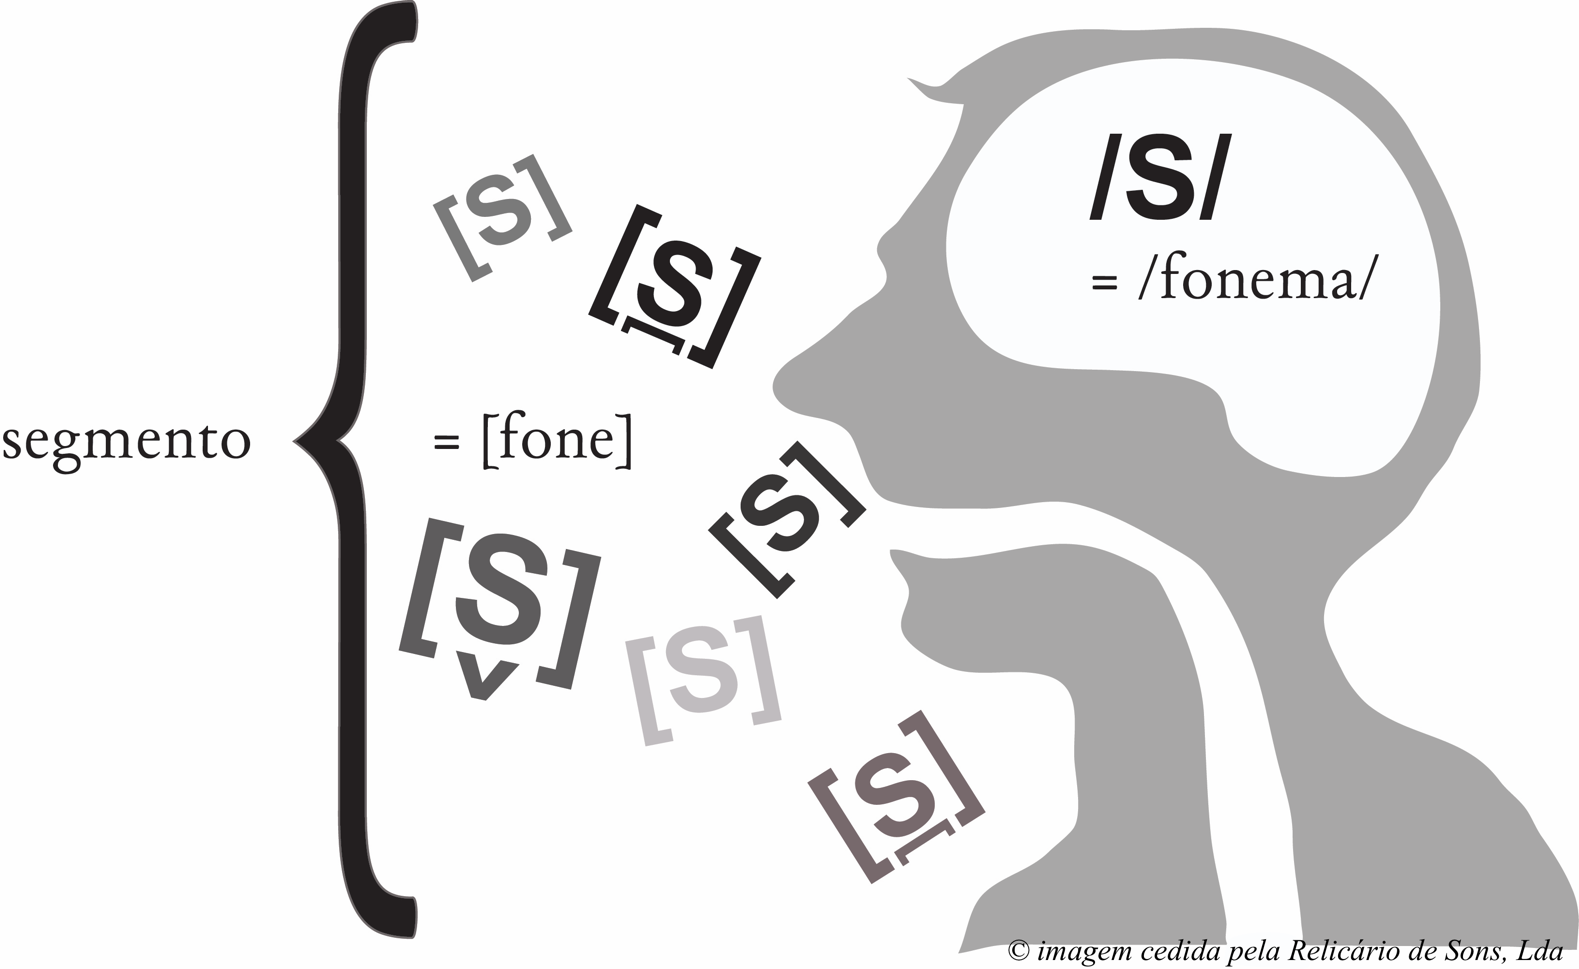
\includegraphics[width=0.75\textwidth]{figures/lousada_fig1}
\caption{Diagrama para distinção entre fone e fonema }
\label{fig:lousada_1}
\end{figure}

Os fonemas e os fones são, assim, unidades de naturezas distintas, com impacto no tratamento da unidade \textit{palavra}, frequentemente usada como estímulo para a \isi{avaliação fonológica} em contexto clínico. Nesta moldura conceptual, as palavras armazenadas no cérebro são concebidas como entradas de um léxico mental, sendo que a representação de cada item lexical contém informação de natureza fonológica, morfológica, sintática, semântica, pragmática (e ortográfica, no caso dos sujeitos alfabetizados). 

Para ilustrar o facto de a informação abstrata representada pelos fonemas ser distinta da informação física associada às formas fonéticas reais, considere-se o caso das palavras j\textipa{[o]}go, j\textipa{[O]}gos, j\textipa{[u]}gador. Um linguista quererá representar, no léxico mental, o facto de estas três palavras serem da mesma família lexical. Para tal, dirá que as três palavras têm o mesmo radical: \textit{jog}-]\textsubscript{RADICAL}. Acontece que a vogal do radical apresenta três formatos fonéticos distintos nas três palavras: \textipa{[o, O, u]} são todas vogais arredondadas mas com alturas distintas. Como é que os linguistas resolvem a diferença entre uma informação homogénea (as três palavras são da mesma família lexical, logo, partilham um mesmo radical) e uma informação heterogénea (as três palavras exibem três vogais com alturas distintas)? Assumem que a vogal representada no léxico mental, o fonema, é uma só, o que permite identificar um mesmo radical para as três palavras e representar, assim, o facto de as três serem da mesma família lexical; as três vogais fonéticas identificadas nas produções das três palavras são fones distintos (neste caso, alofones),\footnote{Usamos fone para designar qualquer som da fala enquanto unidade física (por exemplo, o fonema \textipa{/\textltailn/} está tradicionalmente associado apenas ao fone \textipa{[\textltailn]} em Português europeu); usamos \textit{alofones} para designar dois ou mais sons da fala que estão associados a um mesmo fonema e que decorrem da aplicação de \isi{processos fonológicos}, como no caso ilustrado na Figura \ref{fig:lousada_2}, no texto (para mais informação sobre o assunto, consulte-se \citealt{mateus_etal2005}, secção 5.1).} que resultam de diferentes \isi{processos fonológicos} do Português Europeu (PE) (ver Figura \ref{fig:lousada_2}).

\begin{figure}
\begin{forest}
	[~~~~~~~~~~~~~\textipa{/ZOg-/}\textsubscript{RADICAL}
		[\textipa{[ZOg-]}\textit{os}]
		[\textipa{[Zog-]}\textit{o}]
		[\textipa{[Zug-]}\textit{ador}]
		]	
\end{forest}
\quad
\begin{forest}
	[nível fonológico -- representação mental, no edge [nível fonético -- realidade física, no edge]]
\end{forest}
\caption{Nível fonológico e nível fonético}
\label{fig:lousada_2}
\end{figure}

Referimo-nos à identidade de um segmento através das suas propriedades internas\footnote{Sobre este assunto, consulte-se \citet{mateus_etal2005}, Capítulo 3 e \citet{freitas_etal2012}, secção 3.3.} definidas no domínio da Fonética e tratadas na Fonologia como traços distintivos\footnote{Sobre o conceito de traço distintivo, consulte-se \citet{mateus_etal2005}, secção 5.2.} (por exemplo, a vibração ou não das pregas vocais, identificada na Fonética, é representada por [$+$/$-$ vozeado] na Fonologia).  A \textit{\isi{avaliação fonética}}, pelo tratamento da complexidade motora que lhe é inerente, exige uma tipologia com detalhe descritivo substancial; as tipologias de classificação articulatória contemplam normalmente as seguintes categorias gerais:
\begin{enumerate}[label=(\roman*)]
\item classe principal (consoante, vogal, semivogal);
\item ressonância (oral \textit{versus} nasal);
\item ponto de articulação (bilabial, labiodental, dental, alveolar, palatal, velar, uvular; anterior \textit{versus} posterior);
\item modo de articulação (oclusivas, fricativas, laterais, vibrantes);
\item vozeamento (surdo \textit{versus} sonoro);
\end{enumerate}

No entanto, a \textit{\isi{avaliação fonológica}}, porque lida com a representação de contrastes no conhecimento fonológico e não com motricidade, pode recorrer a um menor número de categorias: a título ilustrativo, as \textit{bilabiais} são sempre \textit{oclusivas} e as \textit{labiodentais} são sempre \textit{fricativas}; a relação entre modo e ponto de articulação permite, assim, construir um sistema de representação mais económico. Evoque-se o caso do ponto de articulação, que necessita de, pelo menos, 7 categorias fonéticas e de apenas 4 categorias fonológicas (ver Tabela \ref{tab:lousada_1}).

\begin{table}
\caption{Ponto de Articulação em PE}
\begin{tabular}{ll}
\lsptoprule
Avaliação fonética & Avaliação fonológica              \\
\midrule
bilabial           & \multirow{2}{*}{labial}           \\
labiodental        &                                   \\
\midrule
dental             & \multirow{2}{*}{coronal anterior} \\
alveolar           &                                   \\
palatal            & coronal posterior                 \\
\midrule
velar              & \multirow{2}{*}{dorsal}           \\
uvular             &                    \\
\lspbottomrule
\end{tabular}
\label{tab:lousada_1}
\end{table}

\subsection{Unidades linguísticas para a análise fonológica}
\label{subsec:lousada_unidades}

Como referido na secção anterior, a \isi{avaliação fonológica} em contexto clínico incide normalmente sobre a unidade \textit{segmento}. Esta tem sido, desde os anos 60 do século passado, a unidade privilegiada para a avaliação clínica e a programação da intervenção. Assim foi também na Fonologia e nos estudos sobre aquisição da linguagem até aos anos 70/80: o segmento era a unidade privilegiada de análise fonológica, sendo tidas em consideração as suas propriedades internas, os traços distintivos. Esta perspetiva de análise é tradicionalmente designada por \textit{Fonologia Linear}. 

A partir dos anos 80, foram identificadas relações entre diferentes tipos de unidades fonológicas, as \textit{unidades segmentais} e as \textit{unidades prosódicas}, passando a ser incorporada, nos vários modelos de representação do conhecimento fonológico, informação sobre as relações entre a unidade \textit{segmento} e as unidades prosódicas, que incluem, entre outras, a \textit{sílaba}, o \textit{acento} e a \textit{palavra prosódica}. Com base nas relações identificadas entre estas unidades, passámos a considerar a existência de vários constituintes fonológicos, hierarquicamente organizados entre si. Esta perspetiva de análise é designada como \textit{Fonologia Não-Linear} (ou \textit{Multilinear}).\footnote{Sobre este assunto, consulte-se \citet{mateus_etal2005}.}

Na sequência deste novo paradigma de análise fonológica, a Fonologia Não-Linear, os estudos em aquisição da fonologia passaram a testar a pertinência destes constituintes para a descrição do desenvolvimento infantil (cf. Capítulos 3, 4 e 5 neste volume), sendo as mais exploradas as relações entre \textit{segmentos} e \textit{constituintes silábicos} (Ataque, Rima, Núcleo e Coda)\footnote{Para informação sobre os constituintes silábicos Ataque, Rima, Núcleo e Coda, consulte-se \citet{mateus_etal2005} e \citet{freitassantos2001}, Capítulo 5.}, \textit{acento de palavra}, \textit{extensão de palavra} e \textit{posição na palavra}. Apesar de a relevância destes aspetos estar amplamente documentada na literatura internacional sobre aquisição da fonologia, a exportação desta perspetiva para a avaliação e a intervenção clínicas \citep{bernhardtstemberger2000} tem tido reduzido impacto nas práticas quotidianas dos terapeutas da fala. Trabalho em curso entre terapeutas da fala e linguistas visa incorporar, na construção de instrumentos de avaliação e de análise, bem como em materiais de intervenção, o conhecimento proveniente da aquisição da fonologia, no sentido de promover o rigor linguístico da avaliação e a eficácia da intervenção. Por outras palavras, o objetivo é responder, de forma empiricamente fundamentada, a aspetos como os abaixo listados, no sentido de testar a sua relevância em contexto de avaliação clínica (Capítulo 4, neste volume):\largerpage

\begin{enumerate}[label=(\roman*)]
\item a aquisição de um dado \textit{segmento} pode depender do \textit{constituinte silábico} a que está associado (um segmento (o \textipa{/l/}, por exemplo) pode já ter sido adquirido em Ataque simples (\textit{\underline{l}eite}) mas não em Coda (\textit{fra\underline{l}da}) e/ou em Ataque ramificado (\textit{f\underline{l}or})?
\item a aquisição de um dado \textit{segmento} pode depender do \textit{acento} de palavra (consoantes em contexto tónico são adquiridas antes de consoantes em contexto átono)?
\item a \textit{extensão de palavra} pode ser um fator (des)promotor da aquisição de um \textit{segmento} (palavras extensas são despromotoras do sucesso na produção)?
\item a \textit{posição na palavra} pode condicionar a aquisição de um \textit{segmento} (posições inicial e final de palavra são potencialmente promotoras da aquisição, por oposição à medial)?
\end{enumerate}

As secções que se seguem debruçar-se-ão sobre a avaliação clínica feita em contexto nacional, relacionando-a com as diretivas internacionais neste domínio profissional e remetendo, sempre que relevante, para a integração de aspetos da Fonologia Não-Linear na prática clínica e na investigação desenvolvida por terapeutas da fala.

\section{Avaliação fonética\is{avaliação fonética}}
\label{sec:lousada_avaliacao_fonet}

De acordo com \cite{broomfielddodd2004}, as PSF podem estar associadas a alterações motoras e/ou cognitivo-linguísticas. Para o entendimento destas últimas, contribui a Fonologia; para a restante, a Fonética.

Tradicionalmente, a Fonética debruça-se sobre três aspetos intervenientes no processo de fala: a articulação, a acústica e a perceção. A Fonética Acústica disponibiliza ferramentas para a análise do sinal acústico da fala, presente durante o processo de produção e de transmissão do evento físico, úteis à avaliação de características temporais e/ou espetrais da fala \citep{perkell1997}. Para \citet{rielysmith2003}, a análise acústica da fala contribui não só para a sua caracterização acústica como também articulatória. Por este motivo, e assumindo que a produção alterada de sons da fala também se reflete nas características acústicas dos mesmos, \citet{kent_etal2010} recorda que a análise acústica da fala contribui para a caracterização articulatória de produções patológicas. 

\largerpage A Fonética Articulatória, por seu turno, é a ciência que se dedica ao estudo dos aspetos articulatórios da fala. O domínio motor da fala desenvolve-se a par do processo de maturação cognitivo-linguística, sensorial e biológica, não estando dependente dos da mastigação e da deglutição \citep{kent2000}. As ferramentas que analisam o processamento motor da fala, isto é, os fatores que contribuem para a sua execução motora e neuromotora (neuromuscular, etc.), constituem-se, portanto, como as mais adequadas ao processo de avaliação da articulação. Como referido anteriormente, a análise acústica contribui para a avaliação do desempenho articulatório \citep{rielysmith2003}, podendo esta ser completada por técnicas imagiológicas como a articulografia, a palatografia, a nasografia, a glotografia, a eletroglotografia, e a ultrassonografia, entre outras \citep{berti2013,llisterri2014}, ou ainda por técnicas métricas como o \textit{índice de inteligibilidade},\is{indice@índice de inteligibilidade} o \textit{\is{debito verbal@débito verbal}débito verbal}, a \textit{\isi{diadococinésia oral}}, a \textit{\isi{estimulabilidade}} e a \textit{percentagem de consoantes\is{percentagem de consoantes corretas} e de vogais corretas}, entre outras.

Assumindo que a informação contida no conhecimento fonológico implícito serve tanto à perceção como à produção, defende-se atualmente que estas capacidades não se desenvolvem separadamente \citep{kent2000,peperkampdupoux2002,smith2006,smith2010}. Para que o sinal acústico da fala, resultante de integração de mecanismos (neuro)cognitivos e (neuro)motores, seja descodificado pelos ouvintes, é necessário considerar o processo percetivo inerente ao ato de fala, recorrendo para tal aos contributos da Fonética Percetiva.  Com efeito, a aquisição das características acústicas dos sons da fala, as suas representações fonéticas e fonológicas e o desempenho motor articulatório desenvolvem-se de modo complementar. Segundo estes autores, o desenvolvimento da articulação ocorre em simbiose com o da perceção, já que a sua maturação se alimenta de propriedades acústicas que a criança perceciona (\textit{ibidem}). Por este motivo, a avaliação\is{avaliação fonética} centra-se habitualmente em aspetos predominantemente articulatórios e na análise acústica. 

A Tabela \ref{tab:lousada_2} explora possíveis conclusões acerca do desempenho articulatório de diferentes quadros clínicos.

Com base na Tabela \ref{tab:lousada_2}, constata-se que, apesar de todos os exemplos fornecidos apresentarem produções diferentes do alvo, nem sempre são consideradas patológicas. A análise fonética deve ser concomitante com a apreciação de outros fatores, nomeadamente clínicos, a fim de melhor distinguir entre as produções típicas as atípicas de uma determinada fase do desenvolvimento. Dentro das atípicas, tanto a Fonética como a Fonologia disponibilizam as ferramentas adequadas para o estabelecimento de diagnósticos diferenciais.

\begin{table}
\caption{Análise fonética da produção articulatória de diferentes quadros clínicos}\label{tab:lousada_2}
\resizebox{\textwidth}{!}{
\begin{tabular}{llp{0.3\textwidth}p{0.5\textwidth}}
\lsptoprule
\multicolumn{2}{l}{Caso}                                                             & Exemplo de produção verbal                                                                           & Possível conclusão de avaliação                                                                                                                                                                        \\
\midrule
\multirow{2}{*}{\rotatebox[origin=c]{90}{Típico}}  & \begin{tabular}[c]{@{}l@{}}A.A.\\ 3;07 anos\end{tabular}  & *\textipa{[\textprimstress \textsubbridge{\bibridge{s}}apu]} para \textipa{[\textprimstress sapu]}                                                                                      & Adequado desenvolvimento das estruturas e função articulatória da produção de \textipa{[s]}, tendo em conta a idade.                                                                                         \\
                         & \begin{tabular}[c]{@{}l@{}}R.A.\\ 7 anos\end{tabular}     & *\textipa{[\textprimstress wup5]} para \textipa{[\textprimstress lup5]}, decorrente de um frénulo lingual curto                                              & Inadequado desenvolvimento das estruturas, com repercussões na função articulatória da produção de \textipa{[l]}, tendo em conta a idade.                                                                    \\
                         \midrule
\multirow{4}{*}{\rotatebox[origin=c]{90}{Atípico}} & \begin{tabular}[c]{@{}l@{}}A.M.\\ 5;08 anos\end{tabular}  & *\textipa{[\textsubbridge{\bibridge{s}}5\textprimstress patu]} para \textipa{[s5\textprimstress patu]}, decorrente de um hábito oral prolongado, como o uso de chucha                   & Inadequado desenvolvimento das estruturas (oclusão dentária) como consequência de um hábito (uso da chucha) e com repercussões na função articulatória da produção de \textipa{[s]}, tendo em conta a idade. \\
                         & \begin{tabular}[c]{@{}l@{}}M.J.\\ 10;03 anos\end{tabular} & *\textipa{[5\textprimstress patu]} para \textipa{s5\textprimstress patu}, decorrente de um traumatismo dentário -- queda de bicicleta                      & Inadequado estado das estruturas (dentição) como consequência de uma lesão adquirida (traumatismo) e com repercussões na função articulatória da produção de \textipa{[s]}, tendo em conta a idade.          \\
                         & \begin{tabular}[c]{@{}l@{}}J.L.\\ 3;02 anos\end{tabular}  & *\textipa{[\textprimstress patu]}, com produção hipotónica de \textipa{[p]}, decorrente de uma lesão neurológica -- parilesia cerebral & Inadequado estado tónus muscular como consequência de uma lesão neurológica (paralisia cerebral) e com repercussões na função articulatória da produção de \textipa{[p]}, tendo em conta a idade.            \\
                         & \begin{tabular}[c]{@{}l@{}}M.R.\\ 4;03 anos\end{tabular}  & *\textipa{[\~{o}\textprimstress vidu]} para \textipa{[o\textprimstress vidu]}, decorrente de fenda palatina                                                      & Incompetência velofaríngea como consequência de uma patologia congénita (fenda palatina) e com repercussões na função articulatória da produção de \textipa{[o]}, tendo em conta a idade     \\
\lspbottomrule
\end{tabular}}
\end{table}

\section{\isi{avaliação fonológica}}
\label{sec:lousada_avaliacao_fonologia}

\subsection{Processos fonológicos\is{processos fonológicos}}
\label{subsec:lousada_processos_fonologicos}

Os \isi{processos fonológicos} ou padrões de erro constituem uma medida frequentemente utilizada para analisar o sistema fonológico da criança. Estes \isi{processos fonológicos} são usualmente categorizados em três grupos: processos de \textit{substituição}\is{processos de substituição} (envolvem a substituição de um segmento por outro), processos dos níveis da \textit{palavra e da sílaba} (afetam a estrutura silábica da palavra-alvo ou a estrutura da palavra) e processos de \textit{assimilação}\is{processos de assimilação} (quando dois elementos se tornam mais semelhantes, usualmente a nível de ponto, modo, vozeamento) \citep{dodd_etal2003,miccioscarpino2008}. 

A Tabela \ref{tab:lousada_3} enquadra os \isi{processos fonológicos} nas principais dimensões do conhecimento fonológico, a prosódica e a segmental. Dentro da prosódica, estão contempladas as unidades palavra e sílaba; na segmental, as unidades segmento e traço distintivo.

A Tabela \ref{tab:lousada_3} estabelece a relação entre os \isi{processos fonológicos} mais usuais na literatura e a unidade fonológica afetada. Por este motivo, no caso da assimilação, a Tabela \ref{tab:lousada_3} apresenta o \textit{segmento} como sendo a unidade afetada, já que a \textit{palavra} corresponde à unidade desencadeadora do processo. Com efeito, as classificações consultadas refletem uma organização que não contempla os critérios ‘causa’ \textit{versus} ‘consequência’. 

A Tabela \ref{tab:lousada_3} apresentada demonstra que os \isi{processos fonológicos} descritos na literatura não só assumem a designação da unidade fonológica afetada (e.g. \textit{processos que afetam o nível da palavra e/ou da sílaba}) como ainda a alteração decorrente do processo em si (e.g., \textit{\isi{processos de substituição}}). Tal oscilação está patente em alguns autores \citep{dodd_etal2003,miccioscarpino2008} e estende-se aos aspetos anteriormente referidos. A monotongação, por exemplo, remete para a consequência do processo, já a assimilação remete para a causa. É exemplo disso a classificação proposta em \citet{ingram1992}.

Tais processos servem diferentes propósitos, quer em termos de caracterização do desenvolvimento fonológico típico, quer atípico. Sabe-se que, durante o desenvolvimento linguístico, a criança recorre a processos para simplificar a sua produção enquanto não possui maturidade suficiente para estabilizar a representação dos alvos fonológicos.
\begin{table}
\resizebox{\textwidth}{!}{%
\begin{tabular}{lllll}
\lsptoprule
\multicolumn{2}{l}{Processos Fonológicos} & \multicolumn{2}{l}{Dimensão Afetada} & Exemplo \\
\midrule
Tipo & Subtipo & Prosódica & Segmental &  \\
Níveis da Palavra e da Sílaba & Omissão de consoante final/coda & X &  & `porco' \ipa{[\pstr poku]} \\
 & Omissão de sílaba átona & X &  & `\textit{chapéu}' \ipa{[\pstr pEw]} \\
 & Redução de grupo consonântico/ataque \textit{ramificado} & X &  & `prato' \ipa{[\pstr patu]} \\
 & Metátese intra-silábica & X &  & `\textit{gravata}' \ipa{[g5R\pstr vat5]} \\
 & Epêntese & X &  & `\textit{prato}' \ipa{[p1\pstr Ratu]} \\
 & Monotongação & X &  & `\textit{dois}' \ipa{[\pstr doS]} \\
Substituição & Anteriorização de fricativas (Despalatalização) &  & X & `\textit{chapéu}' \ipa{[s5\pstr pEw]} \\
 & Anteriorização de oclusivas &  & X & `\textit{cabelo}' \ipa{[t5\pstr belu]} \\
 & Anteriorização de nasais &  & X & `\textit{unha}' \ipa{[\pstr un5]} \\
 & Anteriorização de líquidas &  & X & `\textit{colher}' \ipa{[ku\pstr lER]} \\
 & Posteriorização de fricativas (Palatalização) &  & X & `\textit{vassoura}' \ipa{[v5\pstr SoR5]} \\
 & Posteriorização de oclusivas &  & X & `\textit{pato}' \ipa{[\pstr paku]} \\
 & Posteriorização de nasais &  & X & `\textit{anel}' \ipa{[a\pstr \textltailn El]} \\
 & Posteriorização de líquidas &  & X & `\textit{bolo}' \ipa{[\pstr boLu]} \\
 & Desvozeamento &  & X & `\textit{casa}' \ipa{[\pstr kas5]} \\
 & Oclusão &  & X & `\textit{sala}' \ipa{[\pstr tal5]} \\
 & Substituição de líquidas &  & X & `\textit{peras}' \ipa{[\pstr pel5S]} \\
 & Semi-vocalização de líquidas &  & X & `\textit{bola}' \ipa{[\pstr bOw5]} \\
 & Desnasalização &  & X & `\textit{pente}' \ipa{[\pstr pet]} \\
Assimilação & Harmonia &  & X & `\textit{banana}' \ipa{[m5\pstr n5n5]}\\
\lspbottomrule
\end{tabular}%
}
\caption{Enquadramento dos processos fonológicos nas principais dimensões do conhecimento fonológico.}
\label{tab:lousada_3}
\end{table}



As crianças com PSF de base fonológica \citep{lousada_etal2013} podem apresentar um \textit{atraso} ou uma \textit{\isi{perturbação fonológica}}. As crianças com \textit{atraso fonológico} recorrem a processos típicos correspondentes a etapas anteriores nas crianças com desenvolvimento da linguagem típico. Numa \textit{\isi{perturbação fonológica}}, as crianças usam também \isi{processos fonológicos} considerados \textit{atípicos}, ou seja, processos que ocorrem em menos de 10\% da população com desenvolvimento típico \citep{dodd_etal2003}. O som favorito (e.g., substituir todas as consoantes iniciais por \ipa{[t]}) é um processo atípico para o português europeu e para outras línguas \citep{dodd_etal2003}. A omissão com uso de ataque vazio (\ipa{[\pstr atu]} para ‘gatu’) é um processo usualmente referido como atípico para outras línguas \citep{dodd_etal2003,miccioscarpino2008} mas é natural no português europeu \citep{freitas1997}. 

\subsection{Traços distintivos}
\label{subsec:lousada_tracos}

Uma das tarefas que as crianças têm de realizar durante o processo de desenvolvimento linguístico é a de construir o seu léxico mental; nas entradas lexicais, são armazenadas, entre outros aspetos, as representações fonológicas. Estas representações mentais têm um papel determinante no desenvolvimento fonológico, nomeadamente na aquisição do sistema segmental \citep{fikkert2007}.

Vários autores têm assumido que a estabilização fonológica de um sistema linguístico é gradual, ocorrendo a partir de operações mentais processadas com base em unidades menores do que os fonemas, ou seja, os traços distintivos.\footnote{Sobre este assunto, consulte-se \citet{mateus_etal2005}.} Estes são unidades mínimas de natureza acústica ou articulatória que entram na caracterização de um som \citep{matzenauer2004}. Os traços proporcionam a relação entre a representação cognitiva da informação linguística armazenada na mente/cérebro (neste caso, fonológica) e a sua manifestação física (fonética), sob a forma de enunciados de fala, obedecendo às leis implicacionais que regem a hierarquia dos traços distintivos subjacente à Geometria de Traços \citep{clementshume1995}. Os traços distintivos podem ser considerados tanto no processo de avaliação como no de intervenção terapêutica \citep{mota1996,mota1997}. Para ilustrar este racional, apresenta-se a Tabela \ref{tab:lousada_4}, onde se reúne uma amostra de produções orais de palavras isoladas, do menino M.R., com 7 anos e 8 meses.

\begin{table}
\begin{tabular}{ll}
\lsptoprule
Palavra  & Produção de M. R.        \\
\midrule
\textit{borracha} & \ipa{[bu\pstr \;R as5]}  \\
\textit{camelo}   & \ipa{[t5\pstr melu]}     \\
\textit{colher}   & \ipa{[tu\pstr lE]}       \\
\textit{cadeira}  & \ipa{[t5\pstr b5jR5]}    \\
\textit{laranja}  & \ipa{[l5\pstr R\~{5}z5]} \\
\textit{nata}     & \ipa{[\pstr mat5]}       \\
\textit{gato}     & \ipa{[\pstr batu]}       \\
\textit{queijo}   & \ipa{[\pstr t5jzu]}  \\ 
\lspbottomrule
\end{tabular}
\caption{Amostra de produções orais de M.R (7;08)}
\label{tab:lousada_4}
\end{table}

Face às dificuldades demonstradas, e numa perspetiva articulatória, M.R. apresenta uma \textit{\isi{percentagem de consoantes corretas}}, vulgo PCC (ver secção seguinte), de 48\%, pois 11 dos 21 segmentos consonânticos analisados não estão em conformidade com o alvo, correspondendo a uma percentagem distante do esperado para a sua idade. Numa perspetiva fonológica, e partindo de uma análise por traços distintivos, constata-se que os traços distintivos responsáveis pela caracterização dos segmentos em termos de \textit{modo de articulação} e de \textit{vozeamento} estão estáveis, não se verificando o mesmo quanto aos traços relativos ao \textit{ponto de articulação}, por ainda não apresentarem sinais estáveis de especificação relativamente aos seus pares. Na amostra observada, os traços Labial e Coronal [$\pm$anterior] permutam entre si, e o Dorsal encontra-se ausente no sistema da criança.

No processo de avaliação, quando indevidamente recrutada, a análise articulatória pode revelar-se opaca, como o ilustra o caso de M.R., já que, por consistir numa análise segmental, e, portanto, periférica, todas as classes articulatórias (de modo, de ponto e de vozeamento) aparentam estar afetadas, quando, do ponto de vista fonológico, nem todas apresentam alterações. Por outras palavras, espera-se que uma análise por traços distintivos seja mais sistémica e, portanto, mais transparente. Trata-se de uma análise focada nas propriedades que caracterizam os segmentos, os traços distintivos, permitindo, assim, a identificação das propriedades que se afiguram alteradas e/ou instáveis, independentemente do segmento que afetam. Nessa perspetiva, e tal como referido anteriormente, as dificuldades de M.R. decorrem exclusivamente da instabilidade dos contrastes associados aos traços que caracterizam o ponto de articulação dos segmentos, facto não captado através de uma análise via PCC, que considera o segmento, e não o traço distintivo, como a unidade mínima de análise.

Com base nos estudos centrados no desenvolvimento fonológico a partir de dados da produção, tem sido demonstrado o efeito promotor do distanciamento dos segmentos, em termos dos traços que os distinguem \citep{lamprecht_etal2004,lazzarottovolcao2009,mota1996}. \citet{mota1996,mota1997} demonstra a importância de uma avaliação de natureza implicacional, afirmando que a distância entre traços favorece o desempenho, tanto no desenvolvimento como na reabilitação. Quanto mais traços distintivos estiverem presentes na estimulação, mais precoce e eficiente é o processo de estabilização fonológica. Para \citet{mota1996,mota1997} e \citet{motapereira2001}, tal facto, baseado em pressupostos implicacionais, decorre de um processo de generalização de propriedades fonológicas.


Retomando o caso de M.R. apresentado na Tabela \ref{tab:lousada_4}, e tendo por base os segmentos ausentes no seu inventário (\ipa{/S/} $\rightarrow$ \ipa{[s]}; \ipa{/Z/} $\rightarrow$ \ipa{[z]}; \ipa{/k/} $\rightarrow$ \ipa{[t]}; \ipa{/m/} $\rightarrow$ \ipa{[n]}; \ipa{/L/} $\rightarrow$ \ipa{[l]}; \ipa{/g/} $\rightarrow$ \ipa{[b]}; \ipa{/d/} $\rightarrow$ \ipa{[b]}; \ipa{/R/} $\rightarrow$ ausência de produção) e os pressupostos implicacionais descritos anteriormente, assumir-se-ia que:

\begin{enumerate}
\item a estabilização de \ipa{/m/} decorrerá naturalmente, visto o sistema contrastivo de M.R. já dispor dos traços que determinam a sua realização, nomeadamente de [$+$nasal] (presente em \ipa{[n]}) e de Labial (presente em \ipa{[b]});

\item  a estabilização de \ipa{/Z/} levaria colateralmente à estabilização de \ipa{/S/}, ainda que não estimulando especificamente a produção deste último segmento, dado o traço [$-$vozeado] já se encontrar presente no sistema de M.R. (como, por exemplo, em \ipa{[b]});

\item a estabilização de \ipa{/L/} beneficiará colateralmente da estabilização de \ipa{/Z/} e de \ipa{/S/}, ao disponibilizarem o valor de Coronal [$-$anterior] no sistema  contrastivo de M.R., sabendo que o [$+$lateral] já se encontra disponível (como, por exemplo, em \ipa{[l]});

\item a estabilização de \ipa{/k/} e de \ipa{/g/} decorrerá naturalmente, visto o sistema contrastivo de M.R. já dispor dos traços que determinam a sua realização, nomeadamente de [$-$contínuo; [$\pm$vozeado] (presente em \ipa{[t]} e em \ipa{[b]}) e de Dorsal (presente em \ipa{/\;R/});

\item a estabilização do \ipa{/R/}, contrariamente à dos segmentos anteriores, não depende das especificação de traços – pois M.R. já produz \ipa{/R/} em Ataque simples - mas antes da disponibilização do constituinte silábico Coda.
\end{enumerate}

O Modelo Implicacional de Complexidade de Traços (MICT) \citep{mota1996} baseia-se na proposta de \citet{clements1999} sobre os universais fonológicos e na teoria de inventários fonológicos. Este modelo visa representar as relações existentes entre os traços marcados na aquisição e no desenvolvimento da complexidade segmental. Segundo o MICT, os traços distintivos de uma língua são adquiridos de forma gradual, do menos complexo para o mais complexo, construindo-se, assim, toda a rede segmental do sistema fonológico. Para o Português Europeu, não se conhece proposta congénere, devidamente validada, sendo este um dos modelos implicacionais propostos para o português do Brasil.

\subsection{Complementos à \isi{avaliação fonética} e fonológica\is{avaliação fonológica}}
\label{subsec:lousada_complementos}

Como referido anteriormente, a análise do desempenho articulatório pode ser complementada por técnicas métricas como o \textit{índice de inteligibilidade},\is{indice@índice de inteligibilidade} o \textit{\is{debito verbal@débito verbal}débito verbal}, a \textit{\isi{diadococinésia oral}}, a \textit{\isi{estimulabilidade}} e a \textit{percentagem de consoantes\is{percentagem de consoantes corretas} e de vogais corretas}, entre outras. Não elicitando comportamentos exclusivamente (neuro)motores (estruturais, e portanto periféricos), optámos por descrever estas técnicas na presente secção, dado assumirem também a integração de aspetos funcionais presentes no processo de fala. 

\citet{miller2013} e \citet{pascoe_etal2006} definem \textit{inteligibilidade da fala} como sendo uma fala descodificada com clareza e compreendida sem dificuldade. O cálculo do \textit{índice de inteligibilidade}\is{indice@índice de inteligibilidade} reflete a capacidade de um determinado interlocutor reconhecer as palavras ou frases produzidas por um falante, fora de contexto. Usualmente, são utilizados dois métodos para avaliar a inteligibilidade, tarefas de identificação de palavras ou escalas de likert. Nas tarefas de identificação de palavras, solicita-se ao ouvinte que escreva as palavras das amostras que ouviu. Podem ser utilizadas amostras de palavras isoladas, frases ou fala encadeada, previamente gravadas. Geralmente, calcula-se a percentagem de palavras inteligíveis, verificando-se o número de correspondências entre as respostas dos ouvintes e as palavras produzidas. As escalas de likert são tipicamente usadas com amostras de fala encadeada, podendo solicitar-se ao ouvinte que classifique as amostras (e.g., frases) que ouviu ao longo de um continuum de inteligibilidade (e.g., numa escala de 5 pontos, em que 1 representa ‘completamente ininteligível’ e 5 ‘completamente inteligível’). A inteligibilidade constitui uma medida essencial à monitorização da eficácia da intervenção terapêutica \citep{lousada_etal2014}.

A avaliação do \textit{\is{debito verbal@débito verbal}débito verbal} (número de palavras ou sílabas por minuto) deve considerar a velocidade e a precisão. As crianças com débito elevado ou normal podem omitir sílabas ou segmentos, as crianças com \is{debito verbal@débito verbal}débito verbal reduzido apresentam usualmente uma articulação precisa \citep{bowen2015}. \citet{skinder2000} mostrou que as crianças com melhor precisão segmental tendem a apresentar um débito reduzido, enquanto as crianças com pior precisão segmental falam com um ritmo normal ou elevado. 

A avaliação \textit{diadococinética oral}\is{diadococinésia oral} permite a análise de aspetos relacionados com a “maturação e a integridade neuromotora dos órgãos envolvidos na fala (lábios e língua, por exemplo) por meio da avaliação das habilidades motoras orais.” \citep[131]{paganneveswertzner2010}. A \isi{diadococinésia oral} consiste na capacidade de executar repetições rápidas ou movimentos alternados, com contrações musculares opostas, podendo incluir sequências silenciosas ou repetição de sequências silábicas como \ipa{[pa]}, \ipa{[ta]}, \ipa{[ka]} ou \ipa{[pa\pstr taka]}. O cálculo pode ser feito pela contagem do tempo necessário à produção de determinadas repetições ou pela contagem do número de repetições num determinado período de tempo. 

A \isi{estimulabilidade} reflete a capacidade de a criança corrigir um som da fala mal produzido ou de produzir um som \textit{a priori} ausente do seu inventário, após apresentação do alvo \citep{miccio2002,powellmiccio1996}. É considerada uma medida determinante para a distinção entre os subtipos de PSF (no campo da articulação ou da fonologia), na seleção do fonema alvo de intervenção como até na tomada de decisão quanto à elegibilidade para a intervenção \citep{glaspeystoel2005,lousada_etal2013}. 

A \textit{percentagem de consoantes\is{percentagem de consoantes corretas} e de vogais corretas} é uma ferramenta que tem vindo a ser referida na literatura para análise da produção das crianças. A \textit{Percentagem de Consoantes Corretas} (PCC),\is{percentagem de consoantes corretas} por exemplo, consiste na divisão do número de consoantes produzidas corretamente pelo número total de consoantes, multiplicando por 100 \citep{shribergkwiatkowski1982}. Segundo \citet{lousada_etal2013}, constitui atualmente \textit{uma \isi{medida de resultados}}\footnote{Tradução do inglês\textit{ outcome measure}, proposta por \citet{lousada2012}.} da intervenção terapêutica. \citet{jesus_etal2015} estudaram a PCC em crianças falantes do Português Europeu com desenvolvimento típico, tendo obtido os seguintes valores médios nas diferentes faixas etárias analisadas: 84.7 para crianças com idades compreendidas entre os 3;0 e os 4;0; 90.7 para crianças com idades entre os 4;0 e os 4;06; e 95.1 para crianças com idades entre os 4;06 e os 5;0.

Adicionalmente, e tendo em vista uma análise mais específica da produção das crianças, outras medidas têm sido propostas, nomeadamente, a PCC por ponto e modo de articulação e por vozeamento bem como a percentagem de estruturas silábicas corretas \citep{aguilaretal2002,aguilarserra2006}.

\section{Instrumentos de \isi{avaliação fonética} e/ou fonológica\is{avaliação fonológica} do Português Europeu}
\label{sec:lousada_instru_pt}

Dos vários instrumentos de avaliação articulatória\is{avaliação fonética} e/ ou fonológica\is{avaliação fonológica} disponíveis a nível internacional, salientam-se alguns dos mais citados na literatura \citep{bowen2015}: \textit{Diagnostic Evaluation of Articulation and Phonology} (DEAP) \cite{dodd_etal2002}, \textit{Goldman-Fristoe Test of Articulation-2} \citep{goldmanfristoe2000}, \textit{Khan–Lewis Phonological analysis} (KLPA-2) \citep{khanlewis2002} e \textit{Hodson Assessment of Phonological Patterns} (HAPP-3) \citep{hodson2004}. Nestes instrumentos, o examinador pede à criança para nomear um conjunto de imagens ou objetos e regista a transcrição fonética das respostas obtidas para cada palavra-alvo. Posteriormente, é possível analisar os erros das crianças (usualmente classificando-os em \isi{processos fonológicos}) e obter uma percentagem de ocorrência de cada tipo de erro.

Para o Português Europeu, conhecem-se apenas dois instrumentos de avaliação validados. Um deles proporciona uma análise articulatória, o \textit{\isi{Teste de Articulação Verbal}} (TAV, \citealt{guimaraes_etal2014}), e o outro, uma análise fonética e fonológica, o \textit{\isi{Teste Fonético Fonológico - Avaliação de Linguagem Pré-Escolar}} (TFF-ALPE) \citep{mendes_etal2013}. 

O TAV surge na sua primeira versão em 1996, em substituição do \textit{Teste de Articulação da Escola de Reabilitação de Alcoitão} (TAER), único instrumento em Portugal, e até então, com esta finalidade. Ao fim de 17 anos de existência, surge a primeira edição revista do TAV. Esta versão revista mantém o seu propósito final enquanto instrumento de rastreio rápido e sistemático (tempo médio de aplicação, 10 minutos) da produção oral dos 19 segmentos que constituem o sistema consonântico do Português Europeu, através da nomeação de 37 imagens, sem necessidade de treino específico prévio. O desempenho das crianças é calculado a partir da relação ‘segmentos produzidos \textit{versus} segmentos testados’ e é fornecida numa relação numeral simples e em percentagem de sucesso. Pelas suas características orgânicas e conceptuais,\largerpage o teste permite identificar o tipo de dificuldades apresentadas pelas crianças, sendo as fonéticas mais claramente extraíveis do que as fonológicas, por estas não estarem refletidas na estrutura e na organização da folha de registo proposta, embora estejam parcialmente contempladas nos critérios de base de construção e de revisão do teste. Cabe, portanto, ao aplicador, atender à observação e interpretação destes aspetos específicos ou recorrer a outro teste de avaliação da produção, caso os seus objetivos de análise se foquem especialmente nos aspetos fonológicos.

No TFF-ALPE, as respostas são também obtidas através de uma tarefa de nomeação de 67 imagens. No subteste fonológico, os erros são descritos como \isi{processos fonológicos}, sendo facilmente obtida a percentagem de ocorrência de cada processo usado pela criança. Esta análise é útil para planear a intervenção terapêutica (processos com uma percentagem superior a 40\% são prioritários para a intervenção) e analisar a eficácia da intervenção, quando o instrumento é aplicado antes e após um período de tratamento. O processo de validação do instrumento permitiu obter dados normativos para a idade de aquisição de fonemas e para a idade de desaparecimento de \isi{processos fonológicos} em crianças com desenvolvimento típico \citep{lousada_etal2012,mendes_etal2013}. 

\section{Reflexões finais}
\label{sec:lousada_conclusao}

Embora se complementem, a fonologia e a fonética respondem a necessidades distintas. Como tal, as ferramentas disponibilizadas por estas ciências devem ser criteriosamente selecionadas em função das características dos sujeitos em avaliação. Garantindo esse rigor seletivo, alcançam-se descrições e interpretações mais fidedignas dos casos observados e planeiam-se intervenções mais adequadas e, por conseguinte, mais rápidas e eficazes.

Ao longo dos tempos, assistiu-se a uma oscilação constante entre o predomínio da fonética sobre a fonologia, e \textit{vice-versa}, na interpretação das PSF. Esta dinâmica refletiu-se positiva e negativamente na evolução dos seus contributos. O crescente número de pessoas e de profissionais interessados na matéria, mais ou menos especializados, espoletou a emergência de um leque mais alargado de técnicas, modelos e ferramentas de avaliação e de intervenção, mas também uma maior variação quanto ao rigor dos materiais desenvolvidos, à consistência dos seus objetivos, ao racional do seu construto e à coerência da terminologia adotada ou proposta. Para colmatar esta problemática e promover a utilização dos seus produtos, investigadores provenientes de diferentes áreas científicas (Linguística, Terapia da Fala, Psicologia,\largerpage Neurologia, Otorrinolaringologia, Engenharia, entre outras) defendem práticas de investigação interdisciplinares úteis às comunidades científica, profissional e comunitária e aplicáveis às suas necessidades, mantendo o rigor científico que subjaz a tal tarefa. 





{\sloppy
\printbibliography[heading=subbibliography,notkeyword=this]
}
\end{document}